\documentclass[12pt]{article}
\usepackage[T1]{fontenc}
\usepackage[T1]{polski}
\usepackage[utf8]{inputenc}
\newcommand{\BibTeX}{{\sc Bib}\TeX}
\usepackage{graphicx}
\usepackage{amsfonts}
\usepackage{amsmath}
\usepackage{listings}

\setlength{\textheight}{21cm}
\setlength{\emergencystretch}{3em}

\lstset{basicstyle=\ttfamily\footnotesize, columns=fullflexible, frame=lines,
        showstringspaces=false, breaklines=true}

\title{{\bf Zadanie nr 3 - Wielowarstwowy perceptron i metoda wstecznej propagacji błędu}\linebreak
Inteligentna Analiza Danych}
\author{Jędrzej Małaczyński 264351 \and Jędrzej Kostyk 264339}
\date{27 października 2026}

\begin{document}
\clearpage\maketitle
\thispagestyle{empty}
\newpage
\setcounter{page}{1}
\section{Cel zadania}

Celem zadania było zaimplementowanie algorytmu wstecznej propagacji błędu dla dwuwarstwowej
sieci typu wielowarstwowy perceptron (MLP) o architekturze 4--2--4 i wytrenowanie jej tak, aby
kopiowała na wyjścia swoje wejścia dla czterech wzorców binarnych. Zbadano, czy trening jest
skuteczny z~wejściami obciążającymi (BIAS) w~warstwie wyjściowej i~bez nich, oraz jaką rolę
pełnią te wejścia.

\section{Wstęp teoretyczny}

Sieć ma architekturę z~Rys.~2.3 w~materiałach do wykładu~\cite{wyklad2}: 4 neurony kopiujące
w~warstwie wejściowej, 2 neurony liniowe w~warstwie ukrytej (bez biasu) i~4 neurony sigmoidalne
w~warstwie wyjściowej. Każdy neuron wyjściowy ma dodatkowe wejście $h_3=1$ pochodzące od
neuronu obciążającego:
\begin{equation}
 h_i = \sum_{j=1}^{4} w_{ij}^{(1)} x_j,\ \ i=1,2, \qquad
 y_i = f\Big(\sum_{j=1}^{3} w_{ij}^{(2)} h_j\Big),\ \ i=1,\dots,4,
 \label{eq_forward}
\end{equation}
gdzie $f(s)=1/(1+e^{-s})$ jest funkcją sigmoidalną.
Trening polega na minimalizacji funkcji błędu
$E=\tfrac12\sum_{k}\sum_{i}(z_i^{(k)}-y_i^{(k)})^2$ (wzór 2.1 w~\cite{wyklad2}) metodą
wstecznej propagacji błędu~\cite{rumelhart1986}. Zgodnie z~Algorytmem~2.1 błędy warstw
wynoszą $\delta_i^{(2)}=f'(s_i)(z_i-y_i)$, gdzie $f'(s)=f(s)(1-f(s))$, oraz
$\delta_i^{(1)}=\sum_{k} w_{ki}^{(2)}\delta_k^{(2)}$, a~wagi są korygowane według
$w_{ij}^{(1)} \mathrel{+}= \eta\,\delta_i^{(1)}x_j$ i~$w_{ij}^{(2)} \mathrel{+}= \eta\,\delta_i^{(2)}h_j$.
Algorytm~2.1 opisuje jeden wzorzec, dlatego dla czterech wzorców kroki 3)--9) wykonywano
w~każdej epoce kolejno dla każdego wzorca (korekta po każdym wzorcu), losując kolejność
wzorców w~każdej epoce.

\textbf{Interpretacja zadania.} Sieć 4--2--4 to tzw. koder (\textit{encoder})~\cite{ackley1985}:
musi ,,ścisnąć'' cztery wzorce do dwóch liczb $(h_1,h_2)$ i~odtworzyć je na wyjściu. Wejścia są
wektorami jednostkowymi, więc reprezentacja wzorca $k$ w~warstwie ukrytej to po prostu
$k$-ta kolumna macierzy wag $W^{(1)}$, czyli punkt na płaszczyźnie $(h_1,h_2)$. Neuron wyjściowy $i$
daje $y_i>0{,}5$ wtedy i~tylko wtedy, gdy
\begin{equation}
 w_{i1}^{(2)}h_1 + w_{i2}^{(2)}h_2 + w_{i3}^{(2)} > 0 ,
 \label{eq_line}
\end{equation}
czyli po jednej stronie prostej na płaszczyźnie $(h_1,h_2)$. Do kopiowania wejść prosta neuronu $i$
musi oddzielić punkt wzorca $i$ od punktów pozostałych trzech wzorców. Waga biasu $w_{i3}^{(2)}$
decyduje o~tym, czy prosta może leżeć dowolnie, czy musi przechodzić przez początek układu.

\section{Eksperymenty i wyniki}

Wspólne założenia wszystkich eksperymentów:
\begin{itemize}
 \item zbiór treningowy: 4 wzorce $\mathbf{x}^{(k)}=\mathbf{z}^{(k)}=\mathbf{e}_k$ (wektory jednostkowe),
 \item wagi początkowe losowane z~rozkładu $U(-1,1)$, 20 różnych ziaren generatora (0--19),
 \item $\eta = 0{,}5$ i~$20\,000$ epok (w~eksperymentach 1 i~2), błąd $E$ liczony co 10 epok
       na całym zbiorze,
 \item trening uznano za skuteczny, gdy $|z_i^{(k)}-y_i^{(k)}|<0{,}1$ dla wszystkich wzorców i~wyjść.
\end{itemize}

%%%%%%%%%%%%%%%%%%%%%%%%%%%%%%%%%%%%%%%%%%%%%%%%%%%%%%%%%%%%%%%%%%%%%%%%%%%%%%%%%%%%%%%%%%%%%%%%%%%%%%%%%%%%%%%%%
% PODROZDZIAŁ PT. EKSPERYMENT NR 1
%%%%%%%%%%%%%%%%%%%%%%%%%%%%%%%%%%%%%%%%%%%%%%%%%%%%%%%%%%%%%%%%%%%%%%%%%%%%%%%%%%%%%%%%%%%%%%%%%%%%%%%%%%%%%%%%%

\subsection{Eksperyment nr 1 -- trening sieci z~wejściami obciążającymi}

\subsubsection{Założenia}

Sieć dokładnie taka jak w~treści zadania: neurony wyjściowe mają wejście BIAS ($h_3=1$),
co daje razem $8+12=20$ wag.

\subsubsection{Przebieg}

Przeprowadzono 20 treningów z~różnych wag początkowych. Dla każdego zapisano przebieg błędu $E$,
wyjścia sieci po treningu i~reprezentację wzorców w~warstwie ukrytej.

\subsubsection{Rezultat}

\begin{table}[h!]
 \caption{Wyjścia sieci z~biasem po treningu (ziarno 0); wiersz = wzorzec, kolumna = neuron wyjściowy}
 \centering
 \vspace{0.2cm}
 \begin{tabular}{c c c c c}
  \hline\hline\\[-0.4cm]
  \textbf{Wzorzec} & $y_1$ & $y_2$ & $y_3$ & $y_4$\\[0.1cm]
  \hline
  \textbf{1} & $0{,}998$ & $0{,}006$ & $0{,}005$ & $0{,}000$ \\
  \textbf{2} & $0{,}004$ & $0{,}997$ & $0{,}000$ & $0{,}004$ \\
  \textbf{3} & $0{,}006$ & $0{,}000$ & $0{,}998$ & $0{,}007$ \\
  \textbf{4} & $0{,}000$ & $0{,}005$ & $0{,}004$ & $0{,}997$ \\
  \hline
 \end{tabular}
 \label{tab_ybias}
\end{table}

\noindent Wszystkie 20 treningów zakończyło się sukcesem (Tab.~\ref{tab_sum}). Błąd spadł poniżej
$0{,}01$ po 340--530 epokach (mediana 360), a~po $20\,000$ epokach wynosił ok.~$1{,}2\cdot10^{-4}$.
Wyjścia sieci różnią się od wartości pożądanych o~mniej niż $0{,}01$ (Tab.~\ref{tab_ybias}),
czyli sieć poprawnie kopiuje wejścia na wyjścia.

\begin{table}[h!]
 \caption{Reprezentacja wzorców w~warstwie ukrytej i~wagi neuronów wyjściowych (ziarno 0)}
 \centering
 \vspace{0.2cm}
 \begin{tabular}{c c c c c c}
  \hline\hline\\[-0.4cm]
  \textbf{Wzorzec / neuron} $i$ & $h_1$ & $h_2$ & $w_{i1}^{(2)}$ & $w_{i2}^{(2)}$ & $w_{i3}^{(2)}$ \textbf{(BIAS)}\\[0.1cm]
  \hline
  \textbf{1} & $2{,}06$ & $2{,}06$ & $3{,}21$ & $2{,}03$ & $-4{,}53$ \\
  \textbf{2} & $-2{,}86$ & $4{,}01$ & $-1{,}38$ & $2{,}08$ & $-6{,}51$ \\
  \textbf{3} & $0{,}90$ & $-1{,}71$ & $2{,}69$ & $-3{,}94$ & $-2{,}79$ \\
  \textbf{4} & $-3{,}55$ & $-1{,}73$ & $-2{,}46$ & $-1{,}70$ & $-5{,}70$ \\
  \hline
 \end{tabular}
 \label{tab_wbias}
\end{table}

\begin{figure}[h!]
 \centering
 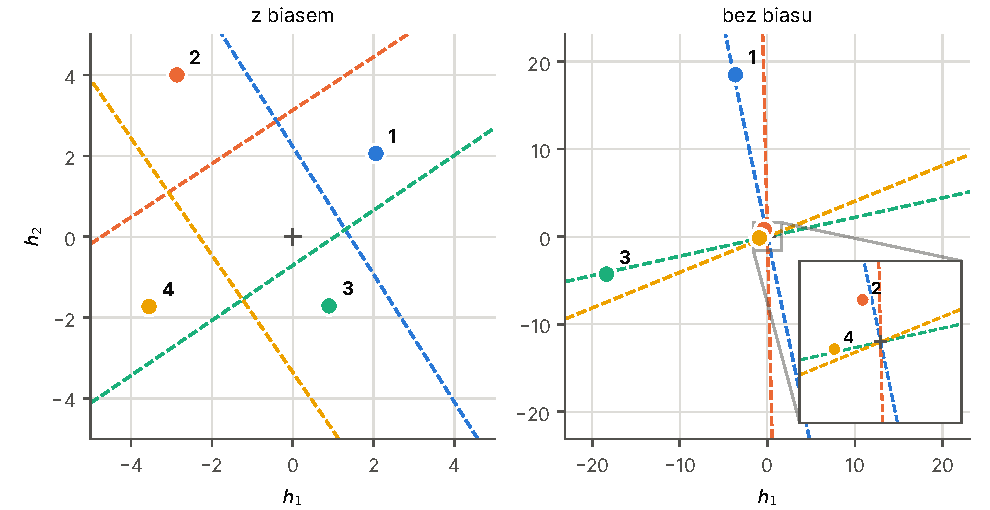
\includegraphics[width=\linewidth]{fig_ukryta.pdf}
 \vspace{-0.6cm}
 \caption{Reprezentacja wzorców 1--4 w~warstwie ukrytej (punkty) i~granice decyzyjne neuronów
 wyjściowych $y_i=0{,}5$ (proste przerywane w~kolorze neuronu), ziarno 0}
 \label{fig_ukryta}
\end{figure}

Rys.~\ref{fig_ukryta} (lewy panel) pokazuje, jak sieć rozwiązała zadanie. Cztery wzorce zostały
zakodowane jako cztery wierzchołki czworokąta na płaszczyźnie $(h_1,h_2)$ (Tab.~\ref{tab_wbias}),
a~prosta każdego neuronu wyjściowego odcina ,,swój'' wierzchołek od trzech pozostałych.
Wszystkie wagi biasu są ujemne (od $-2{,}8$ do $-6{,}5$): bez sygnału z~warstwy ukrytej każdy
neuron wyjściowy jest ,,wyłączony'' ($y_i\approx0$), a~włącza go dopiero reprezentacja jego
własnego wzorca.

%%%%%%%%%%%%%%%%%%%%%%%%%%%%%%%%%%%%%%%%%%%%%%%%%%%%%%%%%%%%%%%%%%%%%%%%%%%%%%%%%%%%%%%%%%%%%%%%%%%%%%%%%%%%%%%%%
% PODROZDZIAŁ PT. EKSPERYMENT NR 2
%%%%%%%%%%%%%%%%%%%%%%%%%%%%%%%%%%%%%%%%%%%%%%%%%%%%%%%%%%%%%%%%%%%%%%%%%%%%%%%%%%%%%%%%%%%%%%%%%%%%%%%%%%%%%%%%%

\newpage
\subsection{Eksperyment nr 2 -- trening sieci bez wejść obciążających}

\subsubsection{Założenia}

Usunięto neuron obciążający, więc $y_i=f(w_{i1}^{(2)}h_1+w_{i2}^{(2)}h_2)$. Sieć ma 16 wag,
a~pozostałe parametry są takie same jak w~eksperymencie nr~1.

\subsubsection{Przebieg}

Wykonano 20 treningów z~tych samych ziaren co w~eksperymencie nr~1. Aby sprawdzić, czy wynik
nie zależy od samej metody treningu, poszukano też minimum funkcji $E$ innym optymalizatorem
(L-BFGS z~biblioteki SciPy, 300 losowych punktów startowych).

\subsubsection{Rezultat}

\begin{table}[h!]
 \caption{Porównanie 20 treningów z~biasem i~bez biasu ($\eta=0{,}5$, $20\,000$ epok)}
 \centering
 \vspace{0.2cm}
 \begin{tabular}{l c c c c c}
  \hline\hline\\[-0.4cm]
  \textbf{Wariant} & $E_{\min}$ & $E_{\textrm{med}}$ & $E_{\max}$ & \textbf{Skuteczne} & \textbf{argmax OK}\\[0.1cm]
  \hline
  z biasem & $1{,}2\cdot10^{-4}$ & $1{,}2\cdot10^{-4}$ & $1{,}2\cdot10^{-4}$ & 20/20 & 20/20 \\
  bez biasu & $0{,}415$ & $0{,}468$ & $0{,}613$ & 0/20 & 20/20 \\
  \hline
 \end{tabular}
 \label{tab_sum}
\end{table}

\begin{table}[h!]
 \caption{Wyjścia sieci bez biasu po treningu (ziarno 0); pogrubiono wartości odbiegające od pożądanych o~co najmniej $0{,}1$}
 \centering
 \vspace{0.2cm}
 \begin{tabular}{c c c c c}
  \hline\hline\\[-0.4cm]
  \textbf{Wzorzec} & $y_1$ & $y_2$ & $y_3$ & $y_4$\\[0.1cm]
  \hline
  \textbf{1} & $0{,}983$ & $0{,}007$ & $0{,}000$ & $0{,}000$ \\
  \textbf{2} & $0{,}020$ & $\mathbf{0{,}374}$ & $0{,}000$ & $\mathbf{0{,}197}$ \\
  \textbf{3} & $0{,}000$ & $0{,}000$ & $0{,}983$ & $0{,}010$ \\
  \textbf{4} & $0{,}000$ & $\mathbf{0{,}198}$ & $\mathbf{0{,}210}$ & $\mathbf{0{,}418}$ \\
  \hline
 \end{tabular}
 \label{tab_ynobias}
\end{table}

\begin{figure}[h!]
 \centering
 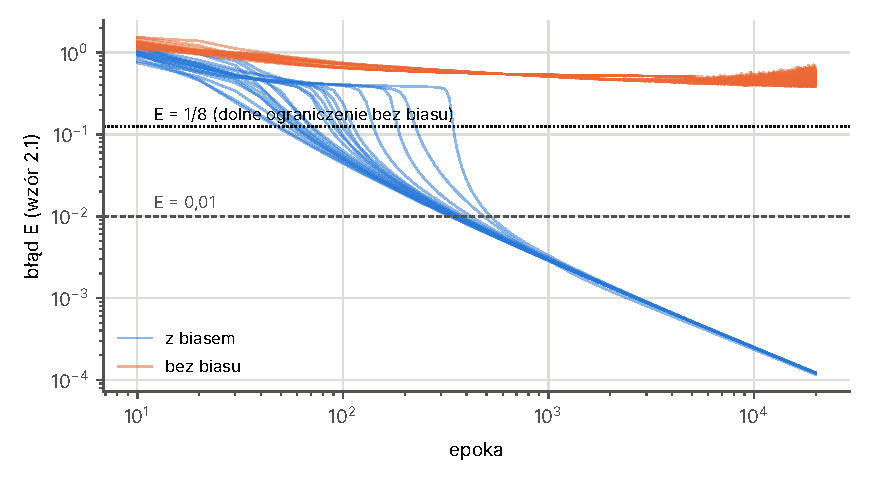
\includegraphics[width=12cm]{fig_bledy.pdf}
 \vspace{-0.3cm}
 \caption{Przebieg błędu $E$ dla 20 treningów z~biasem i~20 treningów bez biasu (osie logarytmiczne)}
 \label{fig_bledy}
\end{figure}

\noindent Bez biasu żaden z~20 treningów nie był skuteczny. Błąd zatrzymał się na poziomie
$0{,}41$--$0{,}61$ (Tab.~\ref{tab_sum}, Rys.~\ref{fig_bledy}) i~pod koniec treningu oscylował,
bo rosnące wagi powodują coraz większe skoki przy korekcie po każdym wzorcu. Typowy wynik
(Tab.~\ref{tab_ynobias}): dwa wzorce są odtwarzane dobrze, a~dla dwóch pozostałych wyjścia
leżą w~okolicy $0{,}2$--$0{,}4$ zamiast $0$ i~$1$. Najmniejszy błąd znaleziony metodą L-BFGS
wyniósł $0{,}258$. Problem nie wynika więc z~algorytmu treningu, tylko z~samej architektury.
Co ciekawe, we wszystkich 20 przypadkach największe wyjście występowało na właściwym neuronie:
sieć ,,wie'', który to wzorzec, ale nie potrafi go odtworzyć.

Wyjaśnia to prawy panel Rys.~\ref{fig_ukryta}. Bez biasu warunek~(\ref{eq_line}) ma postać
$w_{i1}^{(2)}h_1 + w_{i2}^{(2)}h_2 > 0$, więc każda granica decyzyjna musi przechodzić przez
punkt $(0,0)$. Sieć umieściła dwa wzorce daleko od początku układu (dobre odtworzenie), a~dwa
pozostałe blisko niego, gdzie wyjścia są bliskie $f(0)=0{,}5$.

\textbf{Dlaczego zerowy błąd jest niemożliwy.} Gdyby $E<\tfrac18$, to każdy składnik
$\tfrac12(z_i-y_i)^2$ byłby mniejszy od $\tfrac18$, czyli $|z_i-y_i|<\tfrac12$ dla wszystkich
16 par (wzorzec, wyjście). Dla każdego wzorca $k$ musiałaby więc istnieć prosta przez $(0,0)$,
po której jednej stronie leży punkt $\mathbf{h}^{(k)}$, a~po drugiej pozostałe trzy punkty. Trzy
punkty po jednej stronie prostej przez początek układu mieszczą się w~kącie mniejszym niż
$180^\circ$. Uporządkujmy cztery punkty według kąta wokół $(0,0)$. Sąsiednie punkty wyznaczają
cztery luki kątowe o~sumie $360^\circ$. Skoro trzy pozostałe punkty mieszczą się w~kącie mniejszym
niż $180^\circ$, który nie zawiera punktu $k$, to dwie luki przylegające do punktu $k$ sumują się
do ponad $180^\circ$. Po zsumowaniu tego warunku dla wszystkich czterech punktów każda luka jest
liczona dwa razy, co daje $2\cdot360^\circ>4\cdot180^\circ$, czyli sprzeczność. Zatem bez biasu dla dowolnych wag $E\ge\tfrac18$.

%%%%%%%%%%%%%%%%%%%%%%%%%%%%%%%%%%%%%%%%%%%%%%%%%%%%%%%%%%%%%%%%%%%%%%%%%%%%%%%%%%%%%%%%%%%%%%%%%%%%%%%%%%%%%%%%%
% PODROZDZIAŁ PT. EKSPERYMENT NR 3
%%%%%%%%%%%%%%%%%%%%%%%%%%%%%%%%%%%%%%%%%%%%%%%%%%%%%%%%%%%%%%%%%%%%%%%%%%%%%%%%%%%%%%%%%%%%%%%%%%%%%%%%%%%%%%%%%

\newpage
\subsection{Eksperyment nr 3 -- wpływ współczynnika uczenia $\eta$}

\subsubsection{Założenia}

Sieć z~biasem, $\eta\in\{0{,}05;\,0{,}1;\,0{,}2;\,0{,}5;\,1;\,2;\,5\}$, te same 20 ziaren.
Trening przerywano po osiągnięciu $E<0{,}01$ (maksymalnie $20\,000$ epok).

\subsubsection{Przebieg}

Dla każdej wartości $\eta$ zapisano liczbę udanych treningów i~liczbę epok potrzebną do
osiągnięcia $E<0{,}01$.

\subsubsection{Rezultat}

\begin{table}[h!]
 \caption{Liczba epok do osiągnięcia $E<0{,}01$ w~zależności od $\eta$ (20 treningów)}
 \centering
 \vspace{0.2cm}
 \begin{tabular}{c c c c c c}
  \hline\hline\\[-0.4cm]
  $\boldsymbol{\eta}$ & \textbf{Udane} & \textbf{Mediana} & \textbf{Min} & \textbf{Max} & \textbf{Mediana}$\,\cdot\,\eta$\\[0.1cm]
  \hline
  $0{,}05$ & 20/20 & 3559 & 3349 & 5289 & $178$ \\
  $0{,}1$ & 20/20 & 1779 & 1672 & 2641 & $178$ \\
  $0{,}2$ & 20/20 & 889 & 834 & 1316 & $178$ \\
  $0{,}5$ & 20/20 & 356 & 331 & 524 & $178$ \\
  $1{,}0$ & 20/20 & 179 & 163 & 276 & $180$ \\
  $2{,}0$ & 20/20 & 94 & 80 & 178 & $188$ \\
  $5{,}0$ & 17/20 & 55 & 13 & 12298 & $275$ \\
  \hline
 \end{tabular}
 \label{tab_eta}
\end{table}

\begin{figure}[h!]
 \centering
 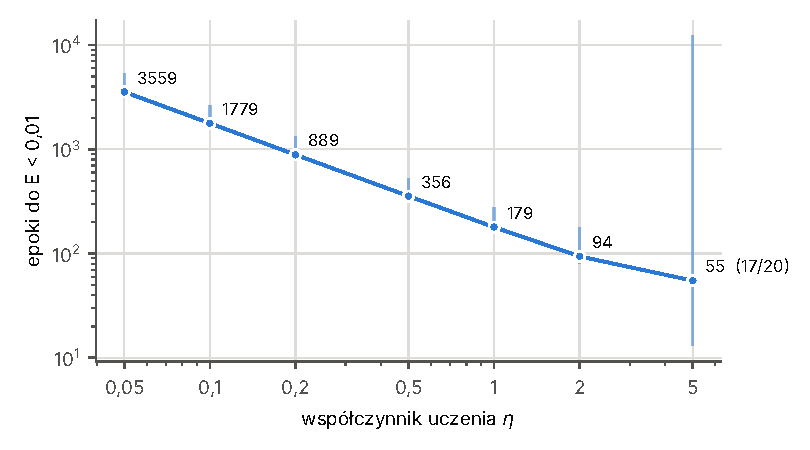
\includegraphics[width=11cm]{fig_eta.pdf}
 \vspace{-0.3cm}
 \caption{Mediana liczby epok do $E<0{,}01$ (pionowe odcinki: zakres min--max) w~funkcji $\eta$}
 \label{fig_eta}
\end{figure}

\noindent Do $\eta=2$ liczba epok jest niemal dokładnie odwrotnie proporcjonalna do $\eta$:
iloczyn mediany epok i~$\eta$ wynosi ok.~$180$ (Tab.~\ref{tab_eta}, Rys.~\ref{fig_eta}).
Dwukrotnie większy krok daje więc dwukrotnie krótszy trening, a~wszystkie treningi kończą się
sukcesem. Przy $\eta=5$ mediana spada już tylko do 55 epok, 3 z~20 treningów nie osiągnęły
$E<0{,}01$, a~jeden potrzebował ponad $12\,000$ epok. Zbyt duży krok sprawia, że korekty
,,przeskakują'' minimum, a~trening staje się niestabilny.

\section{Wnioski}

\begin{enumerate}
 \item Zaimplementowany algorytm wstecznej propagacji błędu (Algorytm~2.1, rozszerzony na wiele
       wzorców) poprawnie trenuje sieć 4--2--4 z~biasem. We wszystkich 20 próbach sieć nauczyła się
       kopiować wejścia na wyjścia z~dokładnością lepszą niż $0{,}01$. Dwa neurony ukryte wystarczają,
       bo cztery wzorce można zakodować jako cztery wierzchołki czworokąta na płaszczyźnie.
 \item Współczynnik uczenia wpływa głównie na szybkość treningu: liczba epok maleje jak $1/\eta$,
       ale przy zbyt dużym $\eta$ (tu 5) trening przestaje być niezawodny.
 \item \textbf{Czy perceptron dałoby się skutecznie wytrenować bez wejść obciążających w~warstwie
       wyjściowej?} Nie. W~żadnym z~20 treningów błąd nie spadł poniżej $0{,}41$, a~najlepszy zestaw
       wag znaleziony niezależnym optymalizatorem daje $E=0{,}258$. Co więcej, pokazano, że dla tej
       architektury bez biasu zawsze $E\ge\tfrac18$. Bez biasu granica decyzyjna każdego neuronu
       wyjściowego musi przechodzić przez początek układu w~przestrzeni $(h_1,h_2)$, a~czterech punktów
       na płaszczyźnie nie da się tak ułożyć, żeby każdy z~nich dało się oddzielić od pozostałych
       prostą przez $(0,0)$. Sieć bez biasu potrafi jedynie wskazać właściwy wzorzec największym
       wyjściem, ale nie odtwarza wartości $0$ i~$1$.
 \item \textbf{Jak intuicyjnie rozumieć rolę biasu?} Bias to regulowany próg zadziałania neuronu,
       podobnie jak wyraz wolny $b$ w~prostej $y=ax+b$: bez niego prosta musi przechodzić przez
       początek układu, z~nim można ją dowolnie przesunąć. Neuron sigmoidalny bez biasu przy zerowym
       sygnale wejściowym zawsze daje $f(0)=0{,}5$, czyli jest ,,niezdecydowany''. W~tym zadaniu każdy
       neuron wyjściowy ma być wyłączony dla trzech z~czterech wzorców. Bias ustawia więc
       ,,domyślną'' odpowiedź na $0$ (wszystkie wyuczone wagi biasu były ujemne), a~neuron włącza
       się dopiero wtedy, gdy sygnał jego własnego wzorca przekroczy ten próg. Geometrycznie bias
       pozwala przesunąć granicę decyzyjną z~początku układu w~dowolne miejsce, dzięki czemu każdy
       neuron może odciąć ,,swój'' wzorzec od pozostałych.
\end{enumerate}

%%%%%%%%%%%%%%%%%%%%%%%%%%%%%%%%%%%%%%%%%%%%%%%%%%%%%%%%%%%%%%%%%%%%%%%%%%%%%%%%%%%%%%%%%%%%%%%%%%%%%%%%%%%%%%%%%
% PODROZDZIAŁ PT. ZALACZNIKI
%%%%%%%%%%%%%%%%%%%%%%%%%%%%%%%%%%%%%%%%%%%%%%%%%%%%%%%%%%%%%%%%%%%%%%%%%%%%%%%%%%%%%%%%%%%%%%%%%%%%%%%%%%%%%%%%%

\section{Załączniki}

Pełny kod znajduje się w~plikach \texttt{mlp.py}, \texttt{eksperymenty.py} i~\texttt{wykresy.py}.
Poniżej podano kroki 4)--9) Algorytmu~2.1 dla jednego wzorca (\texttt{mlp.py}):
\begin{lstlisting}[language=Python]
def hidden(self, x):
    h = self.W1 @ x                                   # 4) warstwa ukryta (liniowa)
    return np.append(h, 1.0) if self.bias else h     #    h3 = 1 - neuron obciazajacy

def forward(self, x):
    h = self.hidden(x)
    s = self.W2 @ h                                   # 5) sumy wazone warstwy wyjsciowej
    return h, f(s)                                    # 6) wyjscia sigmoidalne

def train_pattern(self, x, z, eta):
    h, y = self.forward(x)
    delta2 = y * (1 - y) * (z - y)                    # 7) bledy warstwy wyjsciowej
    delta1 = self.W2[:, :2].T @ delta2                # 8) propagacja bledow wstecz
    self.W1 += eta * np.outer(delta1, x)              # 9) korekta wag warstwy ukrytej
    self.W2 += eta * np.outer(delta2, h)              #    i wyjsciowej (z waga BIAS)
\end{lstlisting}

%%%%%%%%%%%%%%%%%%%%%%%%%%%%%%%%%%%%%%%%%%%%%%%%%%%%%%%%%%%%%%%%%%%%%%%%%%%%%%%%%%%%%%%%%%%%%%%%%%%%%%%%%%%%%%%%%
% BIBLIOGRAFIA
%%%%%%%%%%%%%%%%%%%%%%%%%%%%%%%%%%%%%%%%%%%%%%%%%%%%%%%%%%%%%%%%%%%%%%%%%%%%%%%%%%%%%%%%%%%%%%%%%%%%%%%%%%%%%%%%%

\renewcommand\refname{Bibliografia}
\bibliographystyle{plain}
\bibliography{bibliografia}

\end{document}
